\documentclass[a4paper]{scrartcl}

% Localization
\usepackage[english]{babel}
\usepackage[T1]{fontenc}
\usepackage[utf8]{inputenc}

% Quotations
\usepackage{dirtytalk}

% PDF-compatible landscape mode
\usepackage{pdflscape}

% Advanced tables
\usepackage{array}
\usepackage{tabularx}

% Fancy tablerules
\usepackage{booktabs}

% Graphics
\usepackage{caption}
\usepackage{subcaption}
\usepackage{graphicx}
\graphicspath{{resources}}

% Decent quotations
\usepackage{csquotes}

% Automatic float barriers to each \section
% \usepackage[section]{placeins}

% Math
\usepackage{amssymb,amsmath,amsfonts}
\usepackage{mathtools}

% Algorithms
\usepackage{algpseudocode}

% SI units
\usepackage[binary-units]{siunitx}

% Clickable links in PDF
\usepackage{hyperref}

\title{33107 - Document Image Processing}
\subtitle{Summary}
\author{Michael Senn}
\date{\today}

\begin{document}

\maketitle % Inserts the title, author and date

\tableofcontents

\begin{abstract}
		This summary is based on the lecture notes and slides. It was created
		for the sole purpose of preparing for an exam, with no focus on
		proof-reading, a coherent structure or being suitable for other people.
		Use at your own discretion.
\end{abstract}

% No summary for lecture 1 (introduction)
\setcounter{section}{1}

\section{Image Processing}

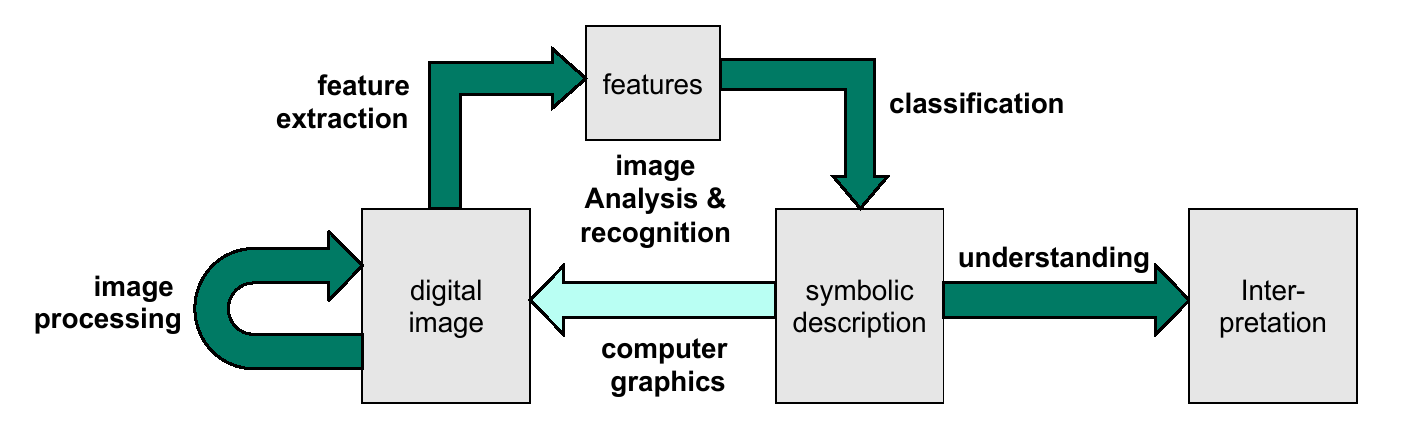
\includegraphics[width=\textwidth]{02_image_disciplines}

\begin{description}
		\item[Image digitalization] Sample to produces pixels, quantize to determine pixel values
		\item[Representation of digital image] Usually as 2D grid.
				Alternatively: Pyramid, with each layer a different resolution.
		\item[Color modes] Direct colour (channels) vs indexed colour (colour map)
		\item[Color spaces] Many different ones
		\item[Quantization] Determine range of pixel values
\end{description}


\subsection{Compression}

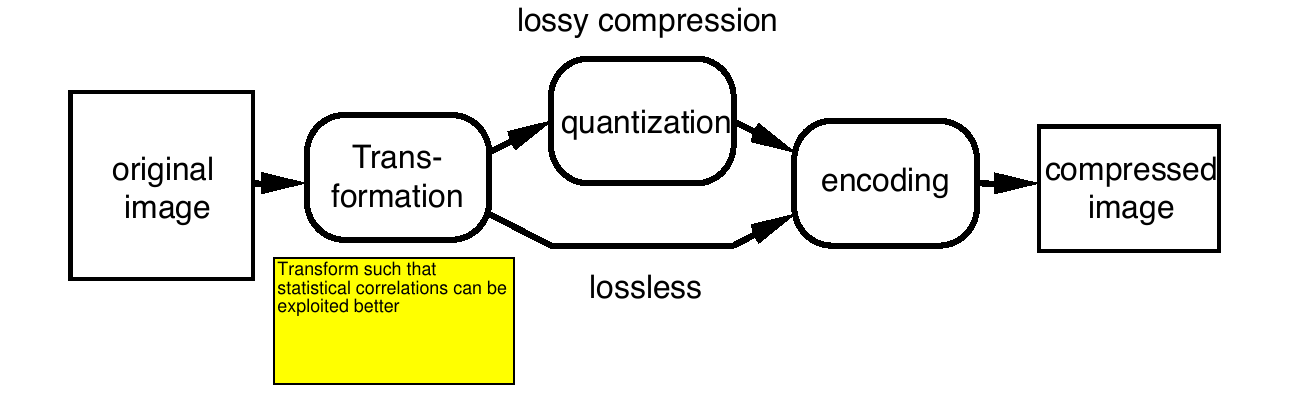
\includegraphics[width=\textwidth]{02_compression}

\begin{itemize}
		\item Lossy vs lossless
		\item Entropy $H(x) = - \sum_{i=1}^n p(i) \log_2(p(i))$. Maximal $H(x)
				= \log_2(n)$ iff all states equally likely (eg uniform noise).
				Minimal $H(x) = 0$ if only one state.
		\item Example: Huffman code, quadtree (recursively partition into four
				quadrants until you get homogenous space)
\end{itemize}

\subsection{Processing operations}

\begin{description}
		\item[Point operation] $z = f(u)$, output depends only on corresponding
				pixel of input. Eg colour inversion, threshold, logical
				combinations.
		\item[Local operation] Each output pixel $(x, y)$ depends on
				neighbourhood $V(x, y)$ of source. Eg convolution operations,
				morphological filters, statistical filters.
		\item[Global operation] Output pixel depends on all pixels of source.
\end{description}

\subsubsection{Convolution}

Mathematical operation of two functions $f$, $g$ producing a third function
defined as (for two dimensions):
\begin{align*}
		f(x, y) \cdot g(x, y) = \int_{- \infty}^{\infty} \int_{-
		\infty}^{\infty} f(\alpha, \beta) \cdot g(x - \alpha, y - \beta)
		d\alpha d\beta
\end{align*}

Discrete case of image $I$ with kernel $k$:
\begin{align*}
		(k \cdot I)[x, y] = \sum_{u = -m}^{m} \sum_{v = -n}^n k[u, v] \cdot I[x
		- u, y - v]
\end{align*}

Kernel is a form of weight given to each pixel the corresponding position. NB
horizontall and veritically flipped in this definition.

\begin{itemize}
		\item Convolution is linear, commutative, associative and shift-independent
		\item Convolution separable iff $k = k_x \cdot k_y$. Reduces complexity
				from $O(m \cdot n \cdot w \cdot h)$ to $O((m + n) \cdot w \cdot
				h)$

		\item Can be used to implement e.g. edge detection, gaussian smoothing,
				min/max/median filter
\end{itemize}

\subsubsection{Spatial vs frequency domain}

\begin{itemize}
		\item Can be toggled between with direct (spaitla -> frequency) and
				inverse (frequency -> spatial) fourier transform.
\end{itemize}


\section{Pattern recognition}

Goal: Discover and identify patterns in raw data. A way of reducing information
to find relevant meaning.

Two categories:

\begin{description}
		\item[Regression] Linear or non-linear. Predict one variable based on
				another, e.g. book price based on page count
		\item[Classification] Multi-class / multi-label classification.
				Classify sample based on variables.
\end{description}

Often operates in two stages:

\begin{description}
		\item[Feature extraction] Remove redundancy, pull out relevant information
		\item[Classification] Make decision based on extracted features
\end{description}

Main issue: Variability of data. E.g. not all letter 'g's look the same.

\subsection{Methods}

\begin{description}
		\item[Statistical] Quantitative approach, appropriate for basic
				objects. Boils down to an optimization problem, sensitive to
				noise.
		\item[Structural] Qualitative approach, appropriate for compound
				objects. Boils down to validation of properties, insensitive to
				noise (binary operation, works fully or not at all).
\end{description}

\subsection{Classifiers}

\begin{itemize}
		\item Model trained by features from training data
		\item Then able to classify data
		\item Supervised (labelled) vs unsupervised (unlabelled, model learns classes itself)
\end{itemize}

\subsection{Feature extraction}

\begin{itemize}
		\item Traditional setups extract features by handcrafted algorithms
		\item Chosen to be discriminative between classes and robust, fast to
				calculate and reasonably compact.
		\item In deep learning, tendency is to avoid handcrafted features
\end{itemize}

Possible features for document image analysis:
\begin{itemize}
		\item Global features such as dimensions, center of gravity, ..
		\item HOG, profiles, LBP
		\item Shape context
		\item ...
\end{itemize}

\subsection{Bayesian}

\begin{itemize}
		\item Given a priori probabilities, determine class with maximum a
				posteriori probability.
		\item Optimal decision boundary minimizes reducible error.
\end{itemize}

\begin{align*}
		P(\omega_i | x) & = \frac{p(x | \omega_i) \cdot P(\omega_i)}{p(x)} \\
		p(x) & = \sum_j p(x | \omega_j) \cdot P(\omega_j)
\end{align*}

\subsection{Classification approaches}

\begin{description}
		\item[Generative] Based on class conditional probabilities (?)
		\item[Discriminative] Based on decision boundaries
\end{description}

\begin{itemize}
		\item Discriminant functions can be used to drive decision, such that
				decision is the one where the corresponding discriminant
				function is the largest of all.
		\item Discriminant function $g$ can be replaced by $f \cdot g$ for any
				monotonic function $f$ (if applied to all discriminant
				functions)
		\item In two-class case, $g_1, g_2$ discriminant functions can be
				combined into $g = g_1 - g_2$, with the decision criteria then
				being $\delta_1 \Leftrightarrow g > 0$.
\end{itemize}

\subsection{Evaluation}

Sound methodology required, management of dataset and clearly specified
metrics. Reproducable execution, control of non-deterministic elements.

\begin{description}
		\item[Accuracy] Global accuracy can be meaningless if unbalanced
				classes, as those have little impact
		\item[Confusion matrices]
		\item[Precision, recall] for two-class problems. $Prec = TP / (TP +
				FP)$, $Rec = TP / (TP + FN)$.
		\item[FAR, FRR] $FAR = FP / (FP + FN), FRR = FN / (TP + FN)$
\end{description}


\section{Initial processing steps}

Diverse set of processing tasks: Preprocessing, segmentation, line separatino,
OCR, ...
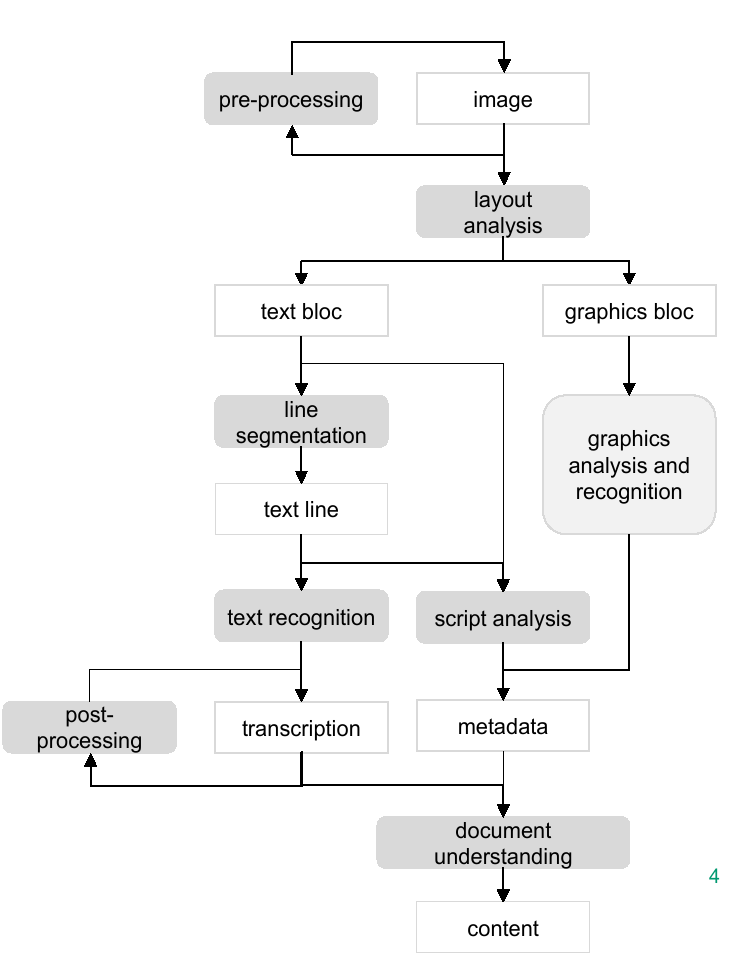
\includegraphics[width=0.5\textwidth]{resources/04_processing_chain}

\subsection{Preprocessing}

Improve quality of images for both visualization as well as processing.
Consists of adjusting resolution, sharpening, colour corrections, deskewing,
binarization, ...

\begin{description}
		\item[Hough transform] skew estimation by mapping pixels to 2D
				parameter space, polar coordinates to estimate skew angle.
		\item[Rotation] can be used to deskew, but introduces distortions
		\item[Bleedthrough] can be removed easily if backside known. Else, use
				gradients.
		\item[Binarization] Global and local operations
\end{description}

\subsection{Layout analysis}

Isolate text blocks, graphics, formula, images, ...

\begin{itemize}
		\item White streams detection recursively does horizontal and vertical
				cuts through white areas. Works well for manhattan layout, less
				well for nested ones. Top-down.
		\item Projectino profiles allow detecting columns or lines, requires
				unskewed image. Top-down.
		\item Connected components, bottom-up aggregation of connected
				components. Useful for binarized printed documents.
		\item Regional classification in e.g. historical documents.
\end{itemize}

\subsection{Text recognition}

\begin{itemize}
		\item OCR suitable for segmented printed text with high-quality images
		\item Handwriting recognition not yet mature, works decently on limited
				vocabulary or when training data available (rather than generic
				model)
		\item Binarization can introduce gaps which lowers OCR performance.
				Context-aware OCR can help, also with similar-looking
				characters.
		\item Sayre's paradox for cursive writing: Character recognition and
				segmentation dependant on each other. Workarounds include
				operations on full words, combining the two, or multiple
				attempts with the most likely one being used.
		\item Depending on alphabet, character recognition (Latin),
				dictionary-based word recognition (Arabic) or stroke
				recognition (Chinese, Japanese) applicable.
\end{itemize}

\subsection{Text alignment}

Align image of text with its transcript. Difficutly depends heavily on accuracy
of transcript and availability of linebreak information.

\subsection{Script analysis}

Script classification, language detection, font recognition, writer
identification, ...

Uses histograms of locale angle distribution, gradients, profiles, run lengths,
...

\subsection{Document understanding}

The last DIA step, first semantic step towards a specific application.
Transformation of physical to logical structure.

\subsubsection{Physical structure}

Publisher's point of view.

\begin{itemize}
		\item Organization of document into regions
		\item Regions into headings and text blocks
		\item Position of figures, separators, ...
\end{itemize}

\subsubsection{Logical structure}

Author's point of view.

\begin{itemize}
		\item Logical structure of document
		\item Articles, titles, headlines, paragraphs, ...
		\item Independent of presentation
\end{itemize}


% No summary for lecture 5 (challenges)
\setcounter{section}{5}

\section{Binary image processing}

\subsection{Binarization}

Goal: Separate foreground and background pixels. Global vs adaptive thresholds.

\subsubsection{Otsu's method}

Minimize threshold of intra-class variance, $p_0 \sigma_0^2 + p_1 \sigma_1^2$,
where $p_i$ is the probability, $\sigma_i^2$ the variance of class $i$.
Equivalent: Maximize inter-class variance $p_0 p_1 (\mu_0 - \mu_1)^2$.

\subsubsection{Niblack's method}

Use local threshold $T_{x, y} = \mu_{x, y} + k \cdot \sigma_{x, y}$, where $k
\in [0, 1]$, typical $k = 0.2$. Window size chosen based on resolution, such
that it contains several characters.

Bad performance if window only includes background!

\subsection{Connected components}

\begin{itemize}
		\item 4-connectivity: Orthogonally connected pixels
		\item 8-connectivity: All neighbouring pixels
		\item n-connected path: Path connected via n-connectivity. E.g.
				4-connected path is akin to movement in Snake, 8-connected path
				akin to movement of queen in chess.
		\item n-connected component IFF for every pair of pixels, there is an
				n-connected path connecting them.
\end{itemize}

\subsection{Jordan's theorem}

In continuous space, a closed simple curve divides the plane into two connected
regions.

In discrete space, a 4-connected curve delimits two 8-connected regions, a
8-connected curve delimits two 4-connected regions.

\subsection{Extracting connected components}

\subsubsection{2D scanning}

Suitable for many small components. Works by only comparing black runs on
current line to those in previous lines. Builds up compoments, merging where
applicable.

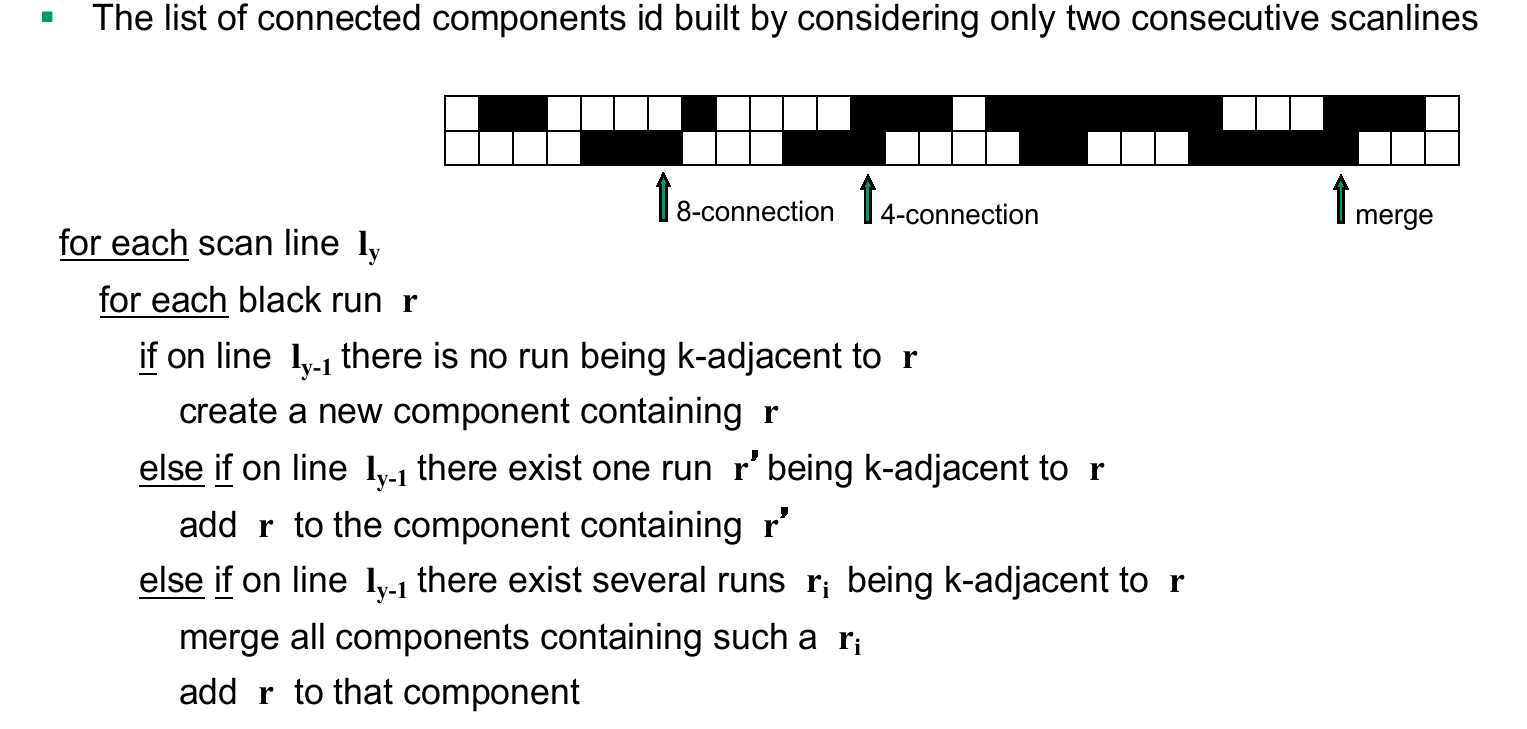
\includegraphics[width=0.5\textwidth]{06_2d_scanning}

\subsubsection{Border following algorithm}

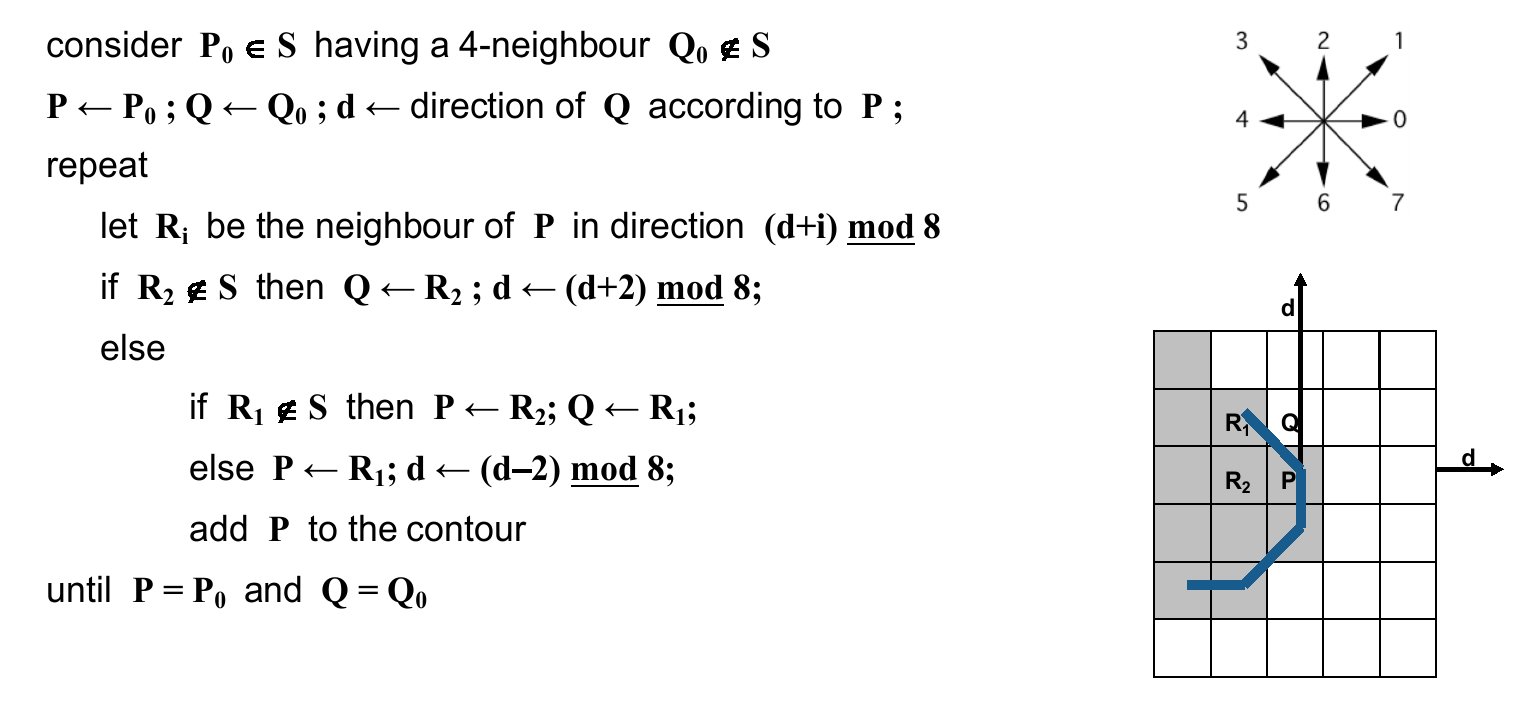
\includegraphics[width=0.5\textwidth]{06_border}

\subsection{Morphological operations}

Operations using a mask (`structurnig element') and an operation, to modify
pixel based on its neighbours. (Local operation).

\subsubsection{Erosion}

Idea: Keep pixels where every pixel of mask has a corresponding pixel on image.
Example mask: Cross shape.

$X \Theta M = \{p | M_p \subset X\}$

\subsubsection{Dilation}

Keep pixels for which any pixel of mask overlaps the shape.

$X \oplus M = \{p | M_p \cap X \neq \emptyset\}$

\subsubsection{Duality of erosion and dilation}

Erosion of inverse is inverse of dilation, and dilation of inverse is inverse
of dilation.

\begin{align*}
		\bar{X} \Theta M = \bar{X \oplus M} \\
		\bar{X} \oplus M = \bar{X \Theta M}
\end{align*}

\subsubsection{Opening and closing}

Let $M^{-}$ be the `symmetric' (mirrored along anchor point) structural
element. If $M$ is symmetric, $M = M^{-}$.

\paragraph{Opening}

Erasion then dilation.

\[
		X \circ M = (X \Theta M) \oplus M^{-}
\]

\paragraph{Closing}

Dilation then erosion.

\[
		X \bullet M = (X \oplus M) \Theta M^{-}
\]

\paragraph{Properties}

\begin{align*}
		\bar{X} \circ M = \bar{X \bullet M}, \bar{X} \bullet M = \bar{X \circ M} && \text{Duality} \\
		X \circ M \subset X, X \subset X \bullet M && \text{Opening is subset, closing is superset of image} \\
		X \subset Y \Rightarrow (X \circ M) \subset (Y \circ M), (X \bullet M) \subset (Y \bullet M) && \text{Monotonically increasing} \\
		(X \circ M) \circ M = X \circ M, (X \bullet M) \bullet M = X \bullet M && \text{Idempotent} \\
		(X \circ M) = \cup \{M_p | M_p \subset X\}
\end{align*}

\subsubsection{Run-length smoothing}

Widely used technique for layout analysis, fill white gaps below a given
threshold horizontally or verticall. Corresponds to opening with $1 \times T$
mask.

\subsubsection{Hit and miss operator}

\[
		\operatorname{ham}_{M_0, M_1}(X) = X \otimes (M_0, M_1) = (X \Theta M_1) \cap (\bar{X} \theta M_0)
\]

Hit and miss operator can be represented as one ternary (three-valued) mask,
where the mask is black where masks one is $1$, white where mask two is $1$,
gray where both masks are white.

\subsubsection{Thinning}

\[
		\operatorname{thin}_M(X) = X - \operatorname{ham}_M(X) = X \cap \bar{(\operatorname{ham}_M(X))}
\]

\subsubsection{Homotopic transformation}

A transformation is homotopic IFF the connexity of all components is preserved,
including wholes. Compare e.g. standard erosion: Can break up components, so is
not homotopic.

Operations can be made homotopic by using special masks.

\subsubsection{Skeleton in euclidean and discrete geometry}

Skeleton $\operatorname{skel}(X)$ of connected component $X$ is all points in
the canters of the maximal inscribed circles. No satisfying of this definition
in discrete space however.

Discrete skeletonization achieved with iterative homotopic transformations,
converting a connected component $X$ into skinny curves.

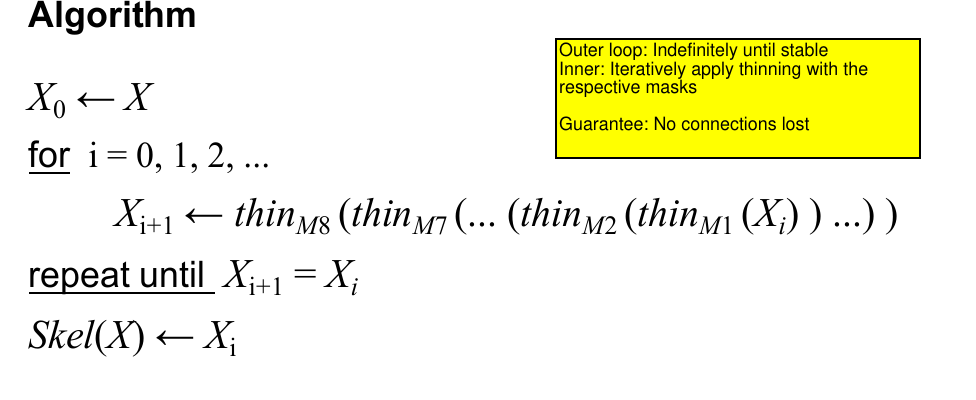
\includegraphics[width=0.5\textwidth]{06_skeletonization}

\subsubsection{Pruning}

Can be used to remove separated pixels after skeletonization. Removes terminal
pixels via hit and miss using certain masks.


\section{Text recognition}

Goal: Transcription (ASCII or Unicode) of text. Analysis also covers language
and script recognition, font recognition, writer authentication, word spotting,
...

OCR good results for non-cursive printed text, clean images, high resolution.
Challenging for cursive script, continuous handwritten text, degraded
documents.

\subsection{Sayre's paradox}

With cursive text / connected characters, character recognition requires
character segmentation, and character segmentation requires character
recognition. Approaches: Recognize whole worlds, test multiple hypothesis,
combine the two.

\subsection{Processing steps}

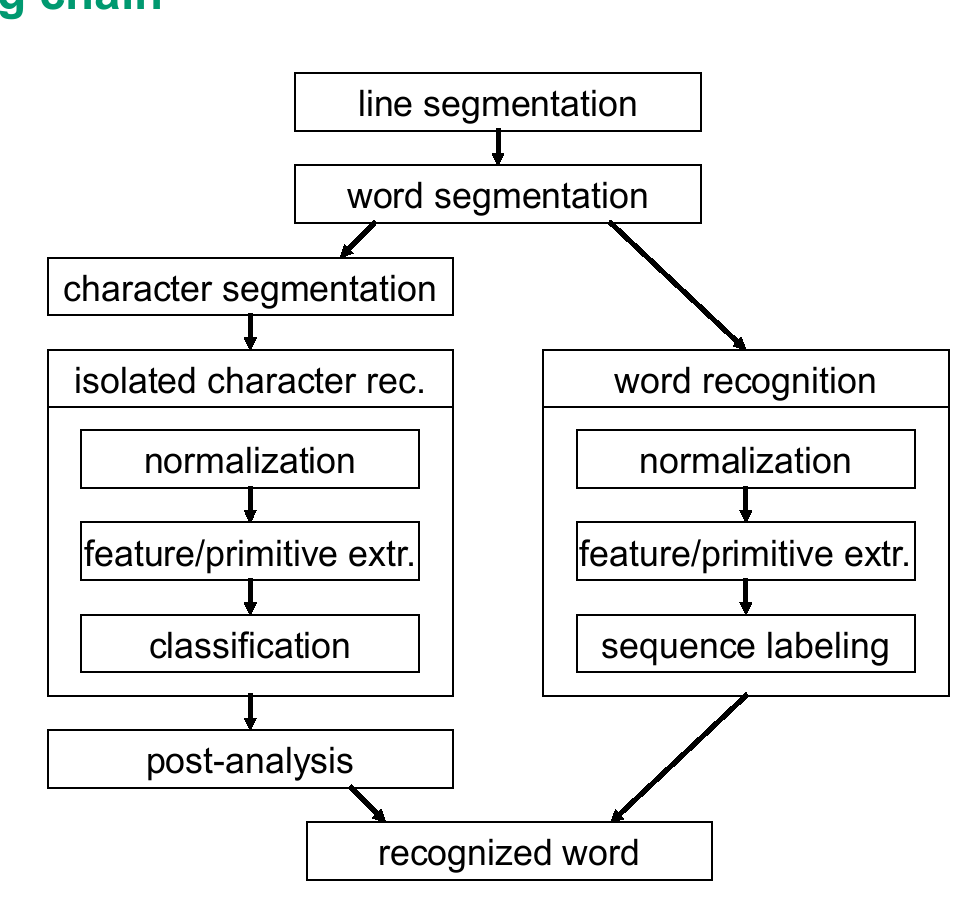
\includegraphics[width=0.5\textwidth]{07_processing}

\subsection{Character recognition}

\begin{itemize}
		\item Isolated character recognition applicable to high-quality printed
				text or constrained handwriting. Challenge: Variability of
				class.
		\item Classification: Statistical (KNN, SVM, ...), direct comparison
				with model, pattern recognition
		\item Similarity measures: Hamming distance, warping distance
		\item Two steps: Feature extraction, then classification
		\item Typical features: Dimensions, density, projection profiles, HOG,
				LBP, ...
\end{itemize}

\subsubsection{Structural approaches}

\begin{itemize}
		\item Shapes decomposed into strokes, properties extracted: Number of
				connected components, number of holes, concavities and
				convexities, ...
		\item These primitives represented as strings, trees, graphs and compared
\end{itemize}

\subsection{Classification}

\begin{description}
		\item[KNN] Sample classified by plurality vote of its neighbours (see
				which class majority of its $k$ nearest neighbours belong to)
		\item[MLP] Fully connected neural network with hidden layer, decision
				based on highest activation on output layer
		\item[SVM] Map initial feature space to augmented space where linear
				discrimination possible. Finds hyperplane with maximum
				separating distance between classes.
\end{description}

\subsection{Word recognition}

\begin{itemize}
		\item Alternative to character recognition, useful if limited
				vocabulary, language-driven approach or keyword spotting
		\item Typically used for cursive scripts, handwriting or
				difficult-to-segment scripts
		\item More possible cases, more features needed
		\item But can use external language knowledge, dictionaries, ...
		\item Feature extraction using sliding window
		\item Dynamic time warping, hidden markov models, ... suitable for
				sequential data analysis
\end{itemize}

\subsubsection{Dynamic time warping}

\begin{itemize}
		\item Calculates similarity between time series, based on DP
\end{itemize}

\subsubsection{Hidden markov model}

\begin{itemize}
		\item Class modeled by a two-stage stochastic process using hidden and
				visible state.
		\item Hidden model has states and transition function (think FSM).
				Observations linked to states via emission functions. Idea:
				Predict state via observations.
		\item That is pick state which best explains patterns in observations.
\end{itemize}


\section{Deep learning}

\begin{itemize}
		\item Machine learning: Decisions determined by a model trained on data
		\item Deep learning: Machine learning based on neural networks
		\item Historically not applicable because of vanishing gradient problem
				(slow convergence), but recent progress due to better
				algorithms, increased processing power and large datasets
\end{itemize}

\subsection{Perceptron}

\begin{itemize}
		\item Calculates weighted sum of inputs
		\item Bias to shift value
		\item Non-linear activation function determines whether output activates or not
\end{itemize}

\[
		\hat{y} = g (w_0 + \sum_{i = 1}^m x_i w_i)
\]

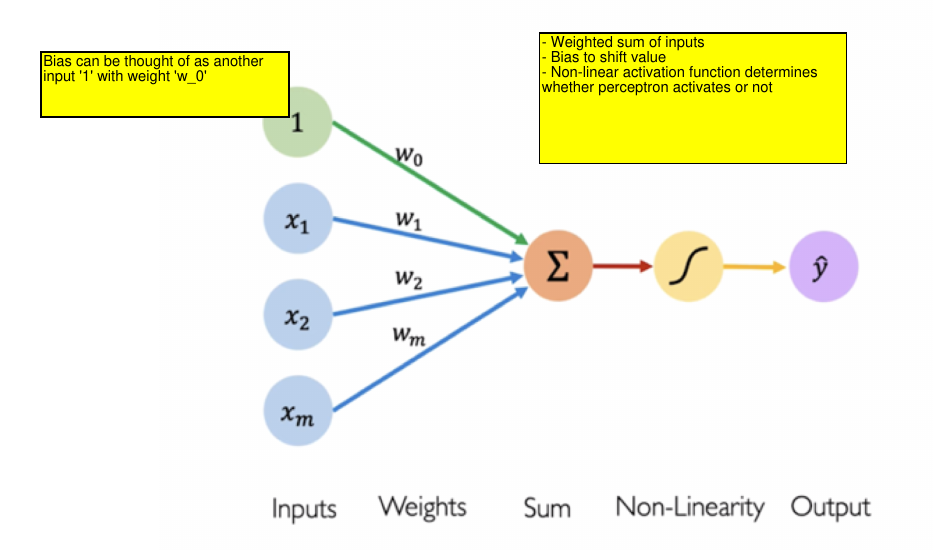
\includegraphics[width=0.7\textwidth]{08_perceptron}

\subsubsection{Common activation functions}

\paragraph{Sigmoid function}

\begin{align*}
		g(z) & = \frac{1}{1 + e^{-z}} \\
		g'(z) & = g(z) \cdot (1 - g(z))
\end{align*}

\paragraph{Hyperbolic tangent}

\begin{align*}
		g(z) & = \frac{e^z - e^{-z}}{e^z + e^{-z}} \\
		g'(z) & = 1 - g(z)^2
\end{align*}

\paragraph{Rectified linear unit}

\begin{align*}
		g(z) & = \max(0, z) \\
		g'(z) & = \left\{\begin{array}{lr}
						1, & \text{for } z > 0 \\
						0, & \text{otherwise} \\
		\end{array}\right.
\end{align*}

\subsection{Single layer neural network}

\begin{itemize}
		\item One hidden layer of perceptrons
		\item Fully connected
		\item One weight matrix per perceptron (with one weight per input each) for input -> hidden transition
		\item And one weight matrix per perceptron for hidden -> output transition
		\item Final outputs are then weighted sums of each perceptron's output,
				again with a weight per perceptron / final output pair, fed
				once more through non-linear activation function.
				\begin{itemize}
						\item Final outputs are effectively perceptrons too,
								which use hidden layer as inputs.
				\end{itemize}
\end{itemize}

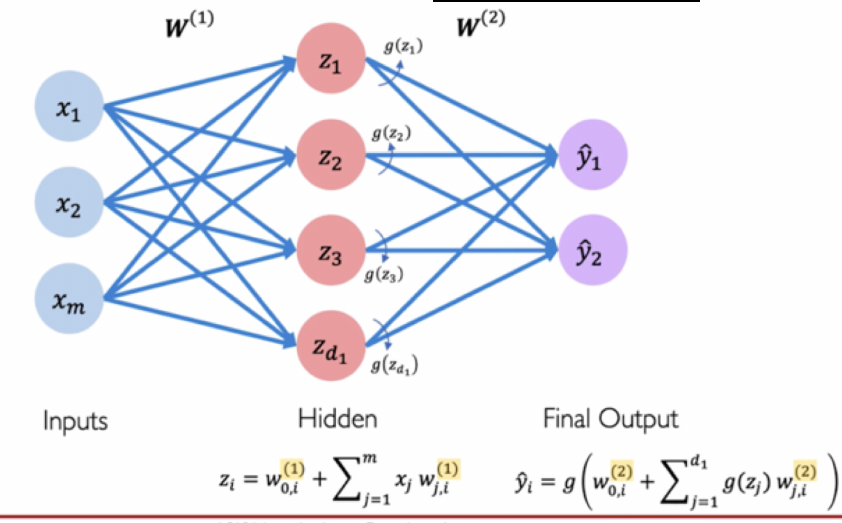
\includegraphics[width=0.7\textwidth]{08_single_layer}

\subsection{Deep neural network}

\begin{itemize}
		\item Many (in practice: several hundred) hidden layers, each consuming
				outputs of previous layer.
\end{itemize}

\subsection{Empirical loss}

\begin{itemize}
		\item Measures total loss over dataset.
		\item `Cost' incurred to network if predicted output incorrect, used to
				train network by making it minimize loss.
		\item During training, network finds weights such as to minimize loss.
\end{itemize}

\begin{align*}
		J(W) = \frac{1}{n} \sum_{i = 1}^n L(f(x^{(i)}; W), y^{(i)})
\end{align*}

Where $x$ inputs, $y$ labels, $f(x)$ predictions, $W = \{W^{(i)}$ weights,
		$J(W)$ total loss, $L()$ loss function, $f(x^{(i)}; W)$ predicted given
		set of weights.

\subsection{Loss optimization}

Find weights $W*$ which achieve lowest loss:

\begin{align*}
		W* = \operatorname{argmin}_W J(W)
\end{align*}

\subsection{Gradient descent}

Move along `down' direction in multidimensional space until convergence.

\subsubsection{Backpropagation}

Problem: How to figure out how to change weights to go `down'? Idea: Use chain
rule to recursively figure out effect changes to weight will have on loss.

Example: Shows how changes to $w_1$ will affect final loss.

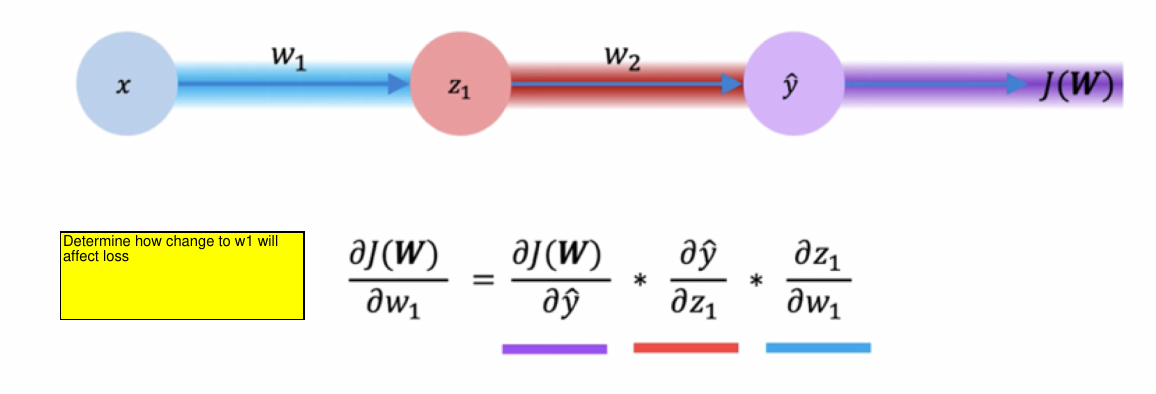
\includegraphics[width=0.7\textwidth]{08_backpropagation}

\subsubsection{Gradient descent algorithm}

\begin{enumerate}
		\item Initialize weights randomly with normal distribution around $0$
		\item Loop until convergence:
				\begin{enumerate}
						\item Compue gradient $\frac{\partial J(W)}{\partial W}$
						\item Update weights $W \coloneqq W - \eta
								\frac{\partial J(W)}{\partial W}$ with learning
								rate $\eta$
				\end{enumerate}
		\item Return weights
\end{enumerate}

\subsubsection{Stochastic gradient descent}

To accelerate convergence: Instead of calculating gradient over full dataset
(costly), use random batch $B$ (order 10s - 100s) over which to calculate
gradient:

\begin{align*}
		\frac{\partial J(W)}{\partial W} = \frac{1}{B} \sum_{k = 1}^B \frac{\partial J_k(W)}{\partial W}
\end{align*}

\subsubsection{Avoiding local minima}

\begin{itemize}
		\item Repeat training with multiple initializations
		\item Adapt learning rates. Too low has risk of being stuck in local
				minima, too high has risk of overshooting.
		\item Less risk of local minima in higher-dimensional spaces.
\end{itemize}

\subsection{Avoiding over-fitting}

\begin{itemize}
		\itemize Dropout: Randomly set certain weights per layer to 0, prevent
				network from becoming too complex
		\item Early stopping: Separate validation set, stop training once
				validation set minimized loss
\end{itemize}


\section{Recurrent neural networks}

\begin{itemize}
		\item Many data sources composed of sequences: Text (of characters),
				sound (time), video (time), signals (time), ..., called
				`sequential data' or `time series'.
		\item Recurrent neural networks designed for such data
\end{itemize}

\subsection{Recap: Feed-forward networks}

Naive approach: Feed sequential data ($k$ points in $t$ sequence entries) as $k
\cdot t$ inputs to feed-forward network. But loses information about which
entries are linked by time step.

\subsection{Neurons with recurrence}

\begin{itemize}
		\item Think of neuron as recurrent cell, which influences itself and is
				fed sequential information in sequence.
		\item Alternatively think of it as sequence of linked neurons, one for
				each time step
		\item Update rules:
				\begin{itemize}
						\item New output depends on \textbf{new state}:
								$\hat{y}^t = W^T_{hy} \cdot h_t$
						\item New state depends on weighted \textbf{past state}
								and weighted \textbf{new input}: $h_t =
								f(W^T_{hh} h^{t-1} + W^T_{xh} x_t)$
				\end{itemize}
		\item Losses from all time steps combined into overall loss
\end{itemize}

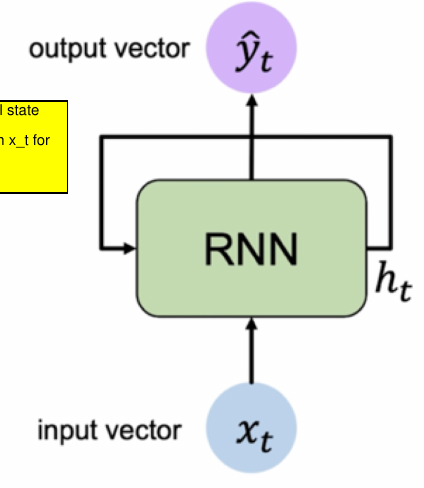
\includegraphics[width=0.5\textwidth]{09_recurrent_cell}

\subsection{Splitting data into sequences}

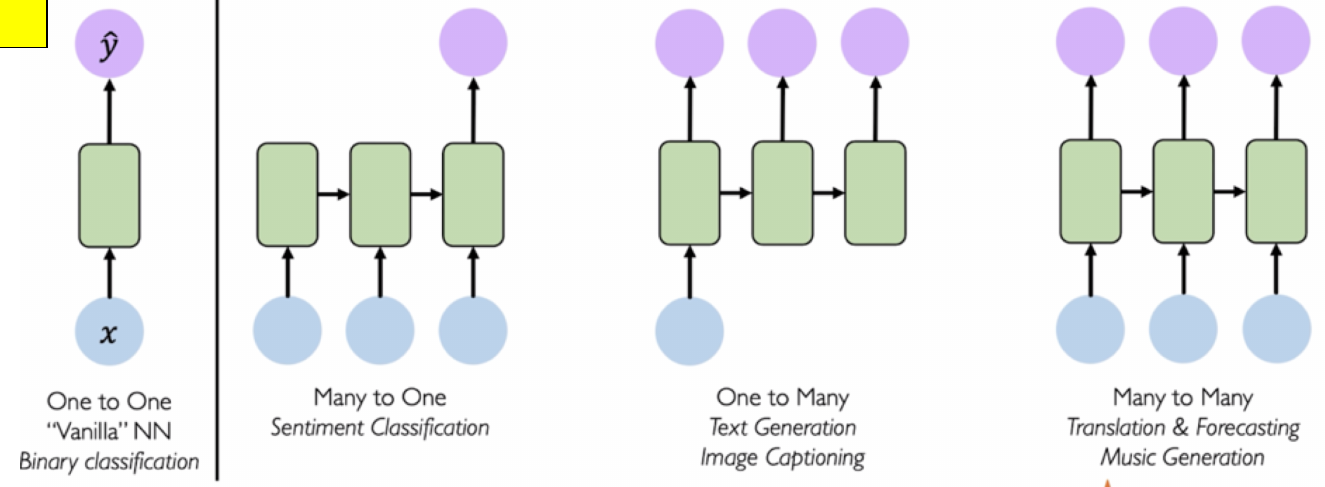
\includegraphics[width=0.7\textwidth]{09_sequential}

Challenges:
\begin{itemize}
		\item Handle variable-length sequences (e.g. sentence length)
		\item Track long-term dependencies
		\item Maintain order information
		\item Share parameters across sequence
\end{itemize}

All fulfilled by RNNs:
\begin{description}
		\item[Variable-length sequences] Map inputs to e.g. fixed-size vectors
				(based on e.g. vocabulary, or sparse vectors)
		\item[Long-term dependencies] RNN uses cell state
		\item[Order information \& shared parameters] inherent
\end{description}

\subsection{Backpropagation}

Backpropagation will go backwards through time.

Gradient contains lots of factors of state-updating weights and gradient
calculation.

\subsection{Exploding gradients}

Many values in gradient $>1$ leads to exploding gradients. Solution: Clipping.

\subsection{Vanishing gradients}

Many values in gradient $< 1$ lead to gradient converging towards $0$, no more
change in model, no more consideration for long-term factors. Multiple solutions:

\begin{itemize}
		\item ReLU as activation function
		\item Diagonal matrices for weights
		\item Gated cells (GRU, LSTM)
\end{itemize}

\subsubsection{Gated cells}

Idea: More complex recurring unit with gates to control what's passed through.
Long short term memory (LSTM) networks rely on gated cell to track information.

Standard repeating module of RNN, with black lines being addition of
weight-matrix weighted factors.

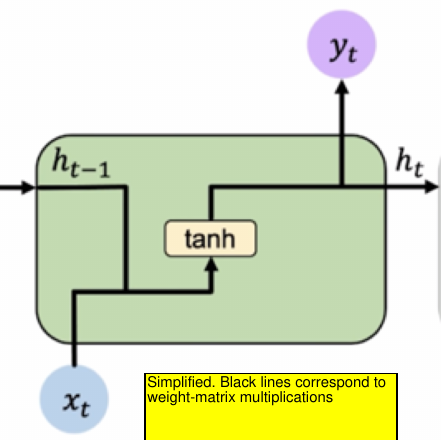
\includegraphics[width=0.5\textwidth]{09_standard_module}

For LSTM: Information added or removed through gates, which selectively let
information pass (by means of e.g. sigmoid function).

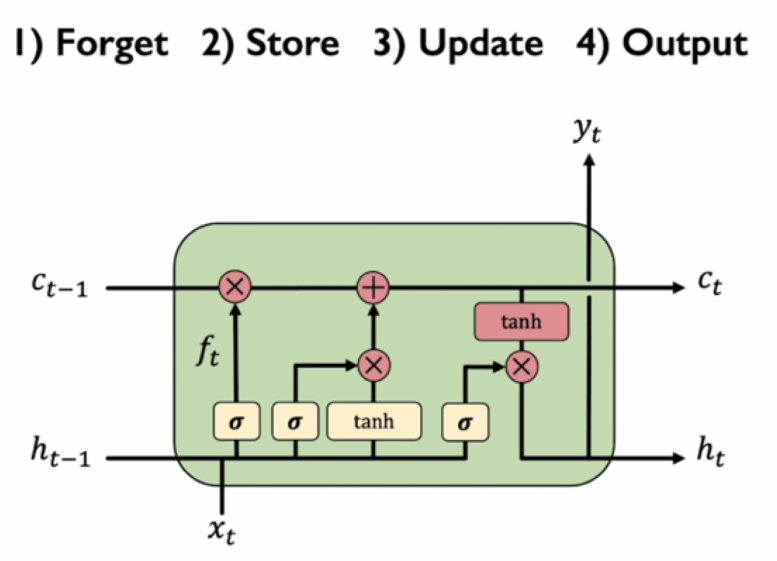
\includegraphics[width=0.5\textwidth]{09_lstm_module}

Implements:
\begin{description}
		\item[Forget] If $h_{t-1} \cdot W + x_t \cdot W$ is small, $f_t$ is
				going to be $0$ Then, $0 \cdot c_{t-1}$ will `forget' the old
				state.
		\item[Store] $\sigma(...) \cdot tanh(...)$ decides whether to store new
				state
		\item[Update] $c_t = (c_{t-1} \times forget) + (store)$ adds new
				information (if there is any worthy of storing) to state ---
				assuming the `forget' gate is not active.
		\item[Output] $h_t = \sigma(h_{t-1} \cdot W + x_t \cdot W) \times
				tanh(c_t)$ is output, also controlled by gate.
\end{description}

Also allows uninterrupted gradient flow - gradient only goes through
easy-to-derive operations.

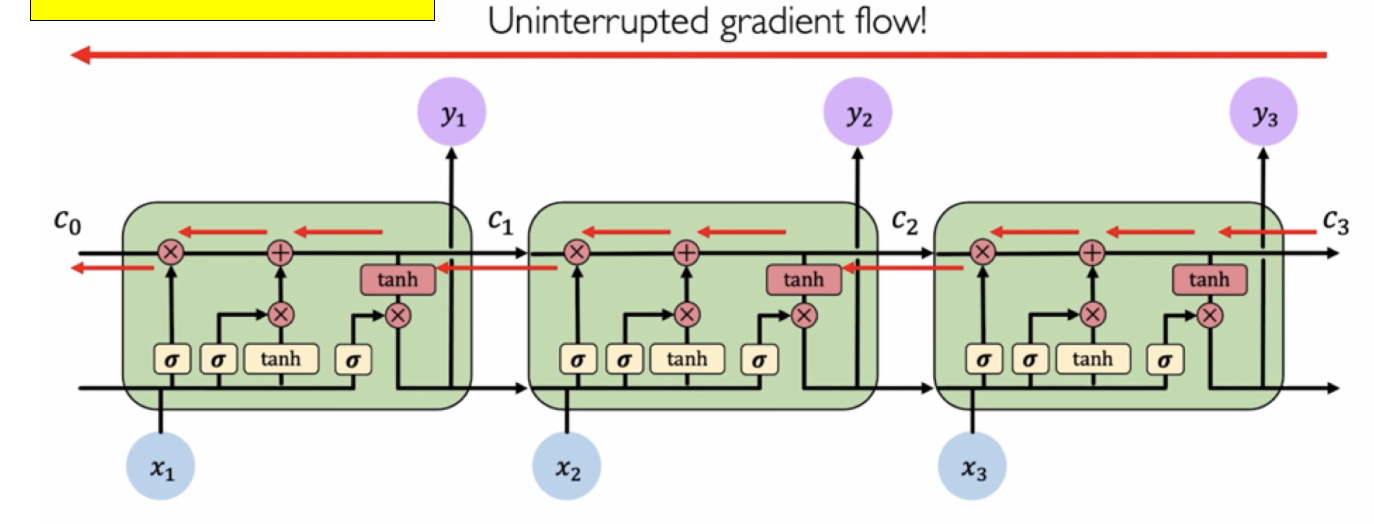
\includegraphics[width=0.7\textwidth]{09_lstm_gradient}


\section{Convolutional neural networks}

Computer vision applied to images (stationary or dynamic), with the goal of
classifying images, detectinb objects and their locations, making predictions,
etc.

Traditional approaches use feature extraction and decision. Issues:
\begin{itemize}
		\item Finding suitable features (suitable for a machine!) is hard
		\item Highly variable data
\end{itemize}

Using fully connected neural networks:
\begin{itemize}
		\item Input is 2D image with spatial information
		\item But fully connected network has every neuron in hidden network
				connected to every neuron in input. Spatial information is
				lost.
		\item And a lot of parameters
\end{itemize}

Approach: Feature extraction with convolution.

\subsection{CNNs for classification}

\begin{enumerate}
		\item Apply convolution filters to generate feature maps
		\item Introduce non-linearity, often with ReLU
		\item Pooling: Downsampling on each feature map
\end{enumerate}

Specifically, each neuron gets only a $x \times y$ window as input.

\subsubsection{Pooling}

Max pool $\max()$ over each pool allows focusing on `positive' aspects of
features.

\subsubsection{Chaining}

Can be chained.

\begin{itemize}
		\item Repeatedly extract features via convolution, activate via ReLU, pooling
		\item Then, flatten feature vectors and feed into fully-connected layer
				for classification
		\item Output is probability of image belonging to a particular class.
\end{itemize}

\subsubsection{R-CNN}

Problem of naive usage of CNNs for object detection: CNN is going to find way
too many objects in each image. Solution: Object detection with R-CNN.

\begin{itemize}
		\item R-CNN algorithm finds regions which might have objects
		\item CNN used on those regions (warped to required dimensions) to find
				and classify objects.
\end{itemize}

\subsection{Semantic segmentation: Fully convolutional network}

\begin{itemize}
		\item FCN is CNN designed with all convolutional layers, including
				downsampling (beginning) and upsampling (end) operations
		\item Model is E2E-trained without human labelling
		\item Pre-trained models can be distributed, requiring only fine-tuning
				with application-specific data.
\end{itemize}


\section{Deep learning for DIA}

Goal: Overview of DIA tasks addressed by deep learning, network architectures
to do so.

\subsection{Autoencoders}

\begin{itemize}
		\item Symmetrical network, trained to recover input from compressed intermediate code
		\item A form of universal feature extractor. Reduces information in a
				way that the `compressed' form is as representative as possible
		\item Outperformed by more specific systems
\end{itemize}

\subsection{Residual neural network}

\begin{itemize}
		\item Convolutional networks with shortcuts to jump over some layers
		\item Shortcuts of length 2 empirically improve performance: Faster
				training, better generalization.
		\item Pretrained networks exist for image analysis
\end{itemize}

\subsection{U-Net}

\begin{itemize}
		\item Several modules, combined by a contracting path (convolutional
				layers, ReLU activation, pooling layers) and expansive path
				(deconvolution).
		\item U-shape. Left half is contracting path, second half is expanding
				path.
\end{itemize}

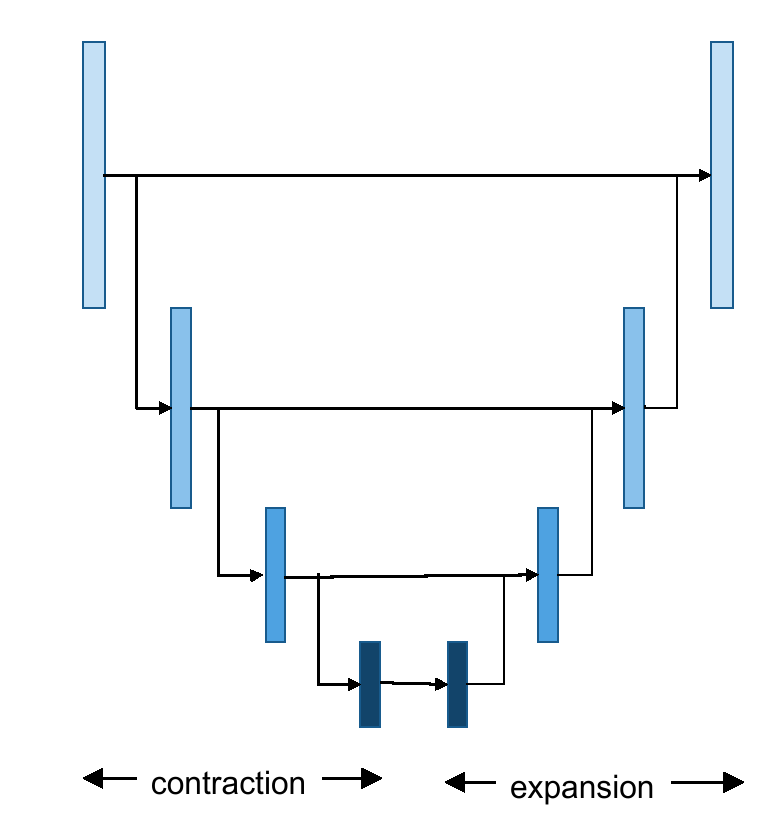
\includegraphics[width=0.5\textwidth]{11_unet}

\subsection{Siamese networks}

\begin{itemize}
		\item Composed of two identical subnetworks with shared weights
		\item Extract feature vector of two similar inputs
		\item Also learn a dissimilarity measure between their two outputs
		\item Well adapted when low amount of data (e.g. signature or face
				recognition)
\end{itemize}

\subsection{Triplet loss function}

\begin{itemize}
		\item Alternative for CNNs, can map input to vector space
		\item Then dissimilarity is measure between vectors in embedded space
		\item Models trained by comparing anchro point with positive and
				engative sample, and minimizing triplet loss function $L(a, p,
				n) = \max(d(a, p) - d(a, n) + margin, 0)$
		\item Anchor $a$ might e.g. be reference image of signature, positive a
				second example, negative a forgery
\end{itemize}

\subsection{GAN}

\begin{itemize}
		\item Used to generate synthetic data
		\item Competing networks, discriminator is trained to distinguish real
				and fake samples, generator is trained to fool the
				discriminator.
		\item Training is computing-intensive and can be tricky
\end{itemize}

\subsection{Semantic layout analysis}

Goal: Detect and classify regions, e.g. background, text blocks, lines,
decorations, ... Different networks:

\begin{description}
		\item[CNN] Sliding window, 3-layer encoder, 1 fully connected hidden
				layer, 1 softmax output layer.
		\item[Asymmetric u-net] 6 convolution layers, 2 deconvolution layers,
				trained with MSE
\end{description}

\subsection{Semantic segmentation}

Goal: Split image into regions. E.g. cat picture into `cat', `sky', `trees',
`grass'.

Approaches:
\begin{description}
		\item[U-Net], evaluation with mean intersection over union: $mIU =
				|C|^{-1} \cdot \sum IU_c$, where $IU_c = \frac{TP_c}{TP_c +
				FP_c + FN_c}$
\end{description}

\subsection{Text line segmentation}

Starting with pixel-wise segmentation, achieve text segmentation of historical
documents.

\subsubsection{Seam carving}

\begin{itemize}
		\item DP, cheapest path through image
		\item Only walk forward, no looking ahead, no backtracking
\end{itemize}

\subsubsection{ML approach}

\begin{enumerate}
		\item Pixel to energy map from segmentation output, text gets high energy, background low energy
		\item Start seam carving every $x$ pixel. Assume seams find lines even
				if they are spaced slightly unevenly
				\begin{itemize}
						\item `Punish' seams for leaving straight path
						\item Release seams from both sides
				\end{itemize}
		\item Collect lines into clusters, generate bins
		\item Get connected components of each bin, connect them with minimum
				spanning three from CC centers, results in (hopefully) one CC
				per line
\end{enumerate}

Evaluation as IoU, average pixel recall and precision, average line recall and
precision.


\section{Signature verification}

\begin{itemize}
		\item Handwritten signatures used for personal authentication
		\item Signature extraction: Find signature within digital image
		\item Signature classification: Identify writer from a set of known
				writers
		\item Signature verification: Determine if signature is genuine from a
				specific writer
\end{itemize}

\subsection{Datasets}

\begin{itemize}
		\item Should cover variabilities due to external factors (pen, ...),
				intrapersonal variability (emotional state, aging, ...),
				interpersonal variability (native script, background, ...)
		\item Many datasets not publicly available due to privacy laws
		\item Datasets often small
		\item Some datasets use generated signatures for training, with small
				real sets for testing
\end{itemize}

\subsubsection{Splitting}

\begin{itemize}
		\item Split approach: Pick first $n$ genuine as reference, then try to
				distinguish remaining genuine from forgeries
\end{itemize}

\subsection{Forgeries}

\begin{description}
		\item[Skilled] Forger has access to genuine signature and time to
				practice. Often of high quality.
		\item[Simple] Forger has access to victim's name. Quality hence depends
				on complexity of genuine signature and forger's luck.
		\item[Random] Forger uses random genuine signature to try and trick
				system.
		\item[Disguised] Writer attempts to modify own signature, for e.g.
				repudiability.
\end{description}

\subsection{Verification system}

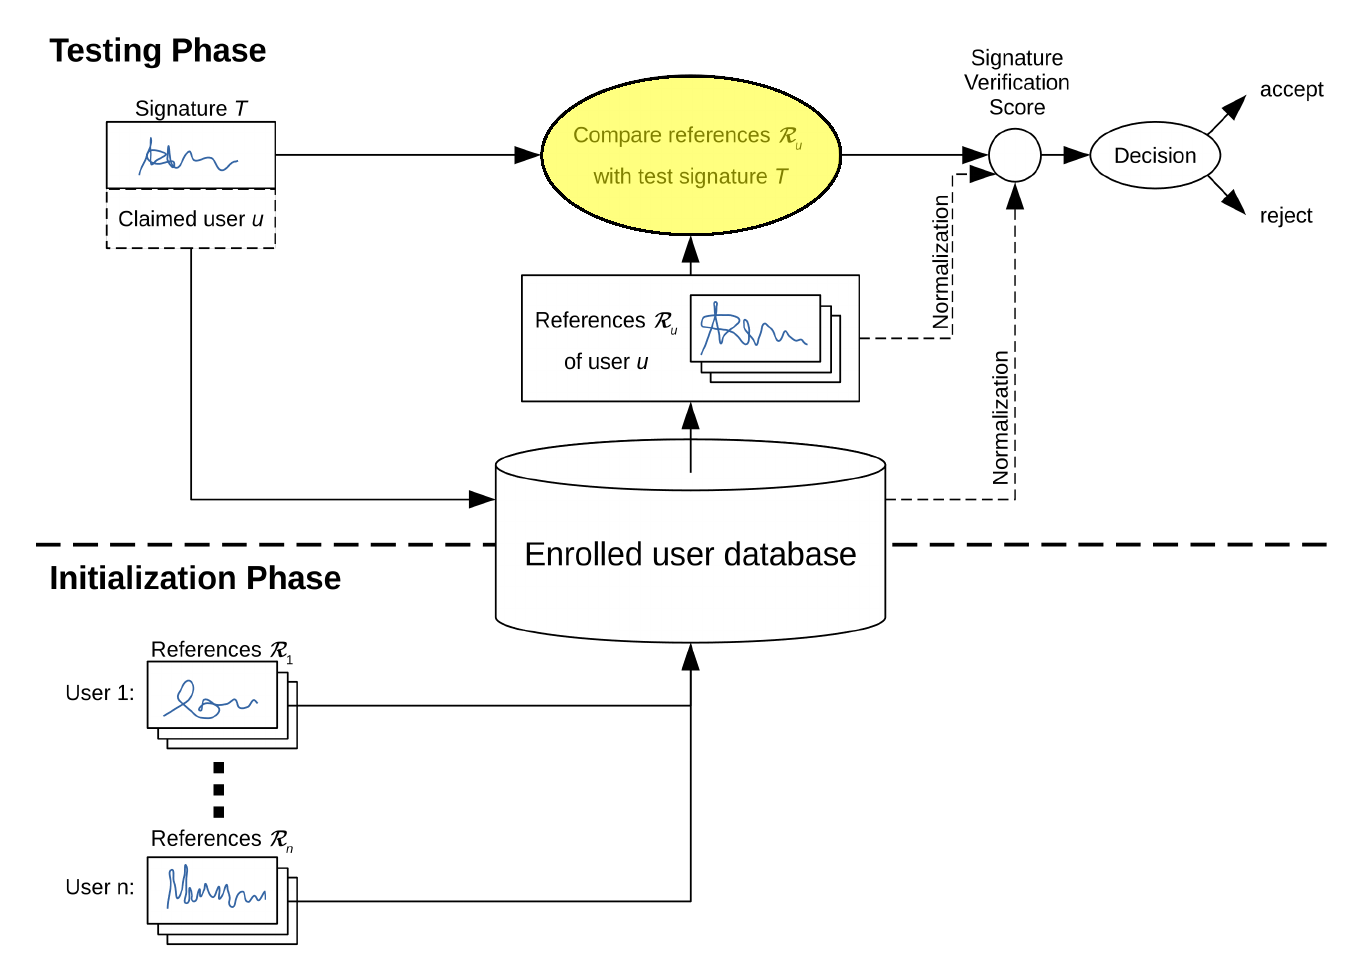
\includegraphics[width=0.7\textwidth]{12_verification_system}

\subsection{Neural network approach}

\begin{itemize}
		\item Extract 128-dimensional feature vector with neural network
		\item Compare those with euclidean distance, use that as dissimilarity
				score
		\item Vector space embedding groups similar signatures
		\item Triplet loss function: Loss based on anchor and positive from
				same user, and negative from another. Random triplets from
				training data. Training minimizes anchor-positive distance
				while maximizing anchor-negative distance.
		\item CNN used as able to utilize spatial information. Two pre-trained
				networks evaluated.
\end{itemize}

\subsubsection{Conlcusion}

\begin{itemize}
		\item Dissimilarity using CNN
		\item Embedding using triplet loss function
		\item Pretraining techniques reduces training cost
\end{itemize}

\subsection{Graph-based approach}

\subsubsection{Approximate signature as graph}

\begin{itemize}
		\item Skeletize via difference-of-gaussian, then binarization.
		\item Then pick points of interest on skeleton, e.g. endpoints, intersectinos, junctions, circles
		\item And evenly spaced points inbetween these
		\item Define graph using those
\end{itemize}

\subsubsection{Graph edit distance}

\begin{itemize}
		\item Minimal cost of transforming one graph into another using a set
				of basic edit operations: Substitution, deleting, insertion of
				nodes and edges.
		\item Each operation has a cost, which is minimized. In this case:
				\begin{itemize}
						\item Node substitution uses euclidean distance between the two
						\item Node insertion / deletion constant cost
						\item Edge substitution no cost
						\item Edge insertion / deletion constant cost
				\end{itemize}
		\item Algorithms solving GED have exponential complexity in number of
				nodes. Even basic signatures with low resolution quickly have
				many nodes!
		\item Two approxmations: Bipartite approximation (BP) with $O(n^3)$,
				Hausdorff Edit Distance (HED) with $O(n^2)$.
\end{itemize}

\paragraph{Bipartite approximation}

\begin{itemize}
		\item Two disjoint sets: Source graph and destination graph
		\item Find bijective mapping between a subset of each
		\item Each node on one side can be assigned to one node on other side,
				or be deleted
		\item Then pick cheapest option
\end{itemize}

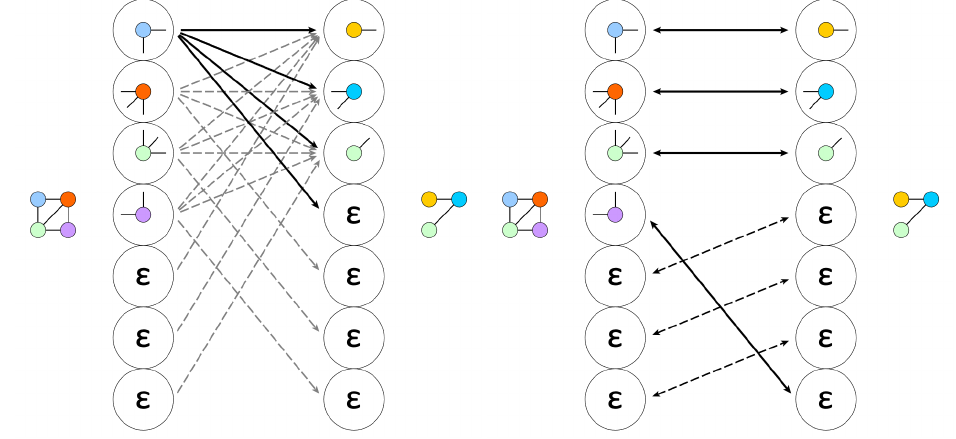
\includegraphics[width=0.6\textwidth]{12_bp}

\paragraph{Hausdorff Edit Distance}

\begin{itemize}
		\item Two sets as above
		\item Allow multiple assignments to same node
\end{itemize}

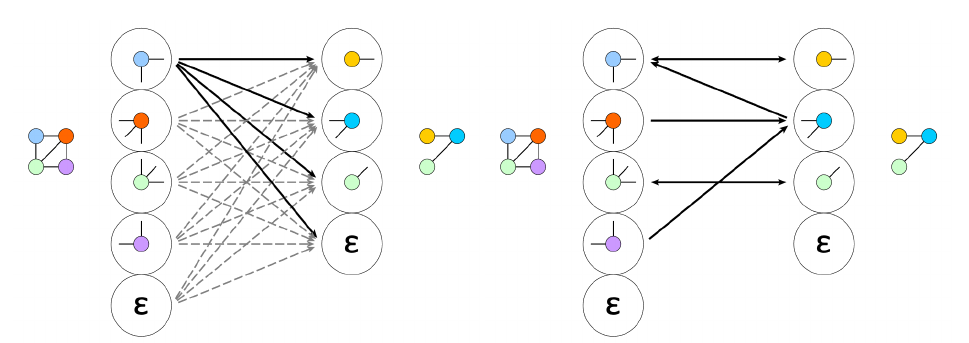
\includegraphics[width=0.6\textwidth]{12_hed}

\subsubsection{GED-based signature dissimilarity}

\[
		d_{GED}(R, T) = \frac{GED(g_R, g_T)}{GED_{max}(g_R, g_T)}
\]

$GED(R, T)$ (approximate) GED between $R, T$. $GED_{max}(R, T)$ is maximum-cost
GED, i.e. deleting all nodes/edges of $R$ and inserting all of $T$, used as
normalization technique. `Naive' edit path which is guaranteed to work.

Results showed that error much lower with normalization!

\paragraph{Results}

\begin{itemize}
		\item HED significantly faster than BP (let alone proper GED) while achieving similar EER
		\item Performance decreases if distance between points on graph gets
				too low (i.e. once approximation too exact, probably as it
				generalizes badly)
\end{itemize}

\subsection{Inkball model approach}

\begin{itemize}
		\item Inkball model is rooted tree
		\item Nodes are points on skeleton, edges to nearest nodes. Label
				specifies position relative to parent node.
		\item Minimize energy cost of tree
		\item Distance again uses normalization term
\end{itemize}

\subsection{Normalization}

\begin{itemize}
		\item User normalization normalizes within data of one user, improves
				performance
		\item Signature verification score normalization to allow combining
				GED, Inkball and CNN dissimilarities
\end{itemize}


\clearpage

\end{document}

